\documentclass[11pt, oneside]{article} 
\usepackage{geometry}
\geometry{letterpaper} 
\usepackage{graphicx}
	
\usepackage{amssymb}
\usepackage{amsmath}
\usepackage{parskip}
\usepackage{color}
\usepackage{hyperref}

\graphicspath{{/Users/telliott//Github/calculus_book/png/}}
% \begin{center} 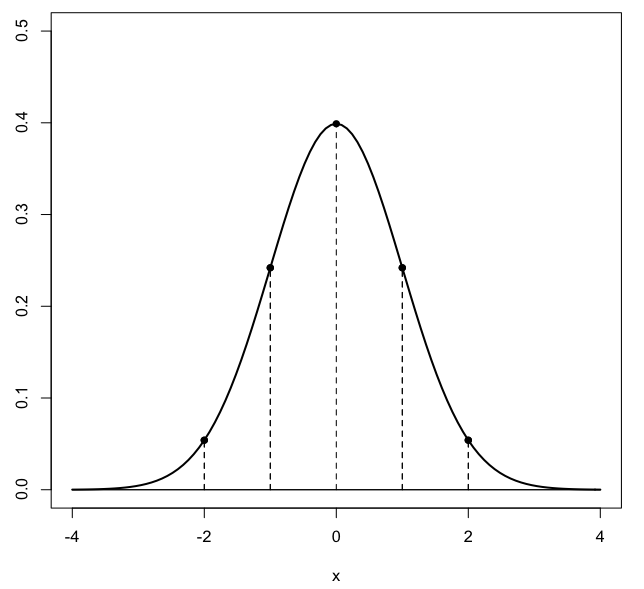
\includegraphics [scale=0.4] {gauss3.png} \end{center}

\title{Circle and cone}
\date{}

\begin{document}
\maketitle
\Large

We needed the formula for the volume of a cone in order to find the volume of a sphere.

Let's start with something simpler, a pyramid.  Consider a cube with all eight edges having length $s$.  So each of the six faces is a square with sides of length $s$ and area $s^2$.

Label the central point inside the solid as $P$.  Draw lines connecting each of the 8 external vertices to $P$, something like this. 
\begin{center}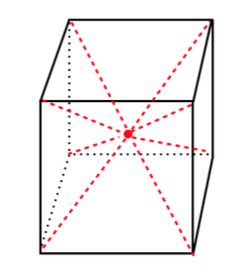
\includegraphics [scale=0.5] {cube_to_cone.png}\end{center}

Now we imagine slicing on planes that connect adjacent pairs of lines.  

You can't do this in real life by slicing up a single cube or rectangular solid, because the cuts to form one surface would ruin some of the other pieces.  The cuts must enter the solid at a corner and then pivot on a line ending at the exact center.  (Perhaps you could do it with a "light saber" since the beam comes to a point).

The result is 6 identical pieces (square pyramids) looking something like this
\begin{center}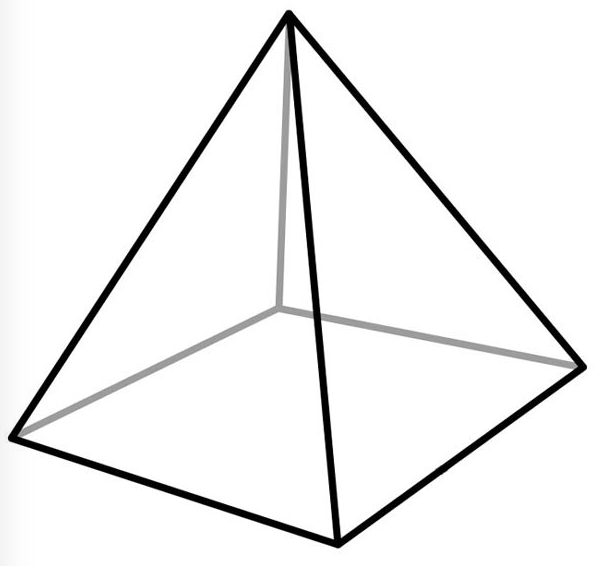
\includegraphics [scale=0.2] {squarepyramid.png}\end{center}

This figure isn't quite accurate because our pyramids will have a height that is $s/2$, but just bear with me.

We started with a cube so that the six resulting solids would be identical.  Unfortunately you can either have six pieces the same, or have some of the pieces with equal base and height, but you can't have both.

Let the six identical pyramid volumes each be $V$, their sum is equal to the volume that we started with.  We have that
\[ 6V = s^3 \]
\[ V = \frac{1}{6} s^3  \]
This is the volume for a pyramid with base area $s^2$ and height $s/2$.  

The volume depends linearly on the height and the area of the base.  The more general formula for a pyramid is really a linear function of $h$
\[ V = \frac{1}{3} hs^2 \]
and you can show this by starting with solids that are longer in one-dimension.

Here is an even better way to slice a cube..

\begin{center}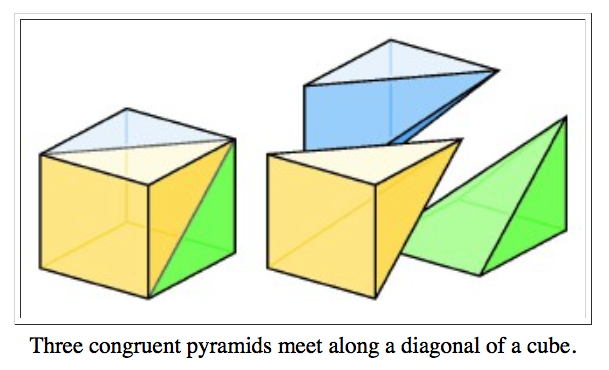
\includegraphics [scale=0.5] {pyramid_cube.png}\end{center}

When I first saw this, I thought it was a trick.  But in fact, we have $3$ identical right square pyramids.

The original cube has 12 edges.  Each pyramid ends up getting three of those edges, all of them meeting at a vertex, plus it has two more edges along the base where there has been a cut, so the edge was shared.

In addition to those, there are two edges where a cut occurred along the diagonal of a face, and then finally the longest edge is (always the same) interior diagonal of the cube.  The total number of edges is $8$.

All three pyramids have a single one of the original external (square) bases, two faces that are one-half of an external face cut along the diagonal, and two faces that were originally internal.  These latter two faces lie along the plane formed between the original interior diagonal axis and the diagonal cuts of the faces.

\url{http://www.math.brown.edu/~banchoff/Beyond3d/chapter2/section02.html}

Of course, a pyramid is not a cone.  But an argument identical to the one we will use for the sphere shows that the volume is independent of the shape of the base.  It just depends on the area.  So for a cone we finally obtain
\[ V =  \frac{1}{3} \pi r^2 h \]

\subsection*{algebraic derivation of the constant 1/3}

I found an algebraic argument on the web at 

\url{https://web.maths.unsw.edu.au/~mikeh/webpapers/paper47.pdf}

Let us assume for this proof that the volume of a cone is proportional to both the area of the base and the height:  $V = cAh$;  our objective is to find the constant of proportionality.

Consider a conical frustum, a cone with the top lopped off.  

\begin{center} 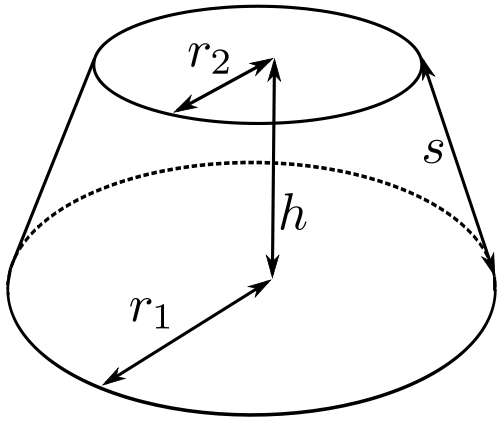
\includegraphics [scale=0.4] {conical_frustum.png} \end{center}

Suppose the area of the base is $A$ and the height of the frustum is $h$.  

Calculate the volume of the frustum as the difference between that of a larger cone with base $A$ and height $h + e$ (e for extra), and that of a small cone with base area $a$ and height $e$.

\[ V = cA(e + h) - cae \]

Now, the area of the base of a cone is $\pi$ times the radius squared, and the radius is proportional to the height (depending on the slant angle).  Hence
\[ a = ke^2 \]
\[ A = k(e + h)^2 \]
so
\[ k = \frac{a}{e^2} =\frac{A}{(e+h)^2} \]
Hence
\[ \frac{\sqrt{a}}{e} = \frac{\sqrt{A}}{e + h} \]

Let us manipulate this expression to find $e$ in terms of $h$:
\[ \frac{\sqrt{A}}{\sqrt{a}} = 1 + \frac{h}{e} \]
\[ \frac{h}{e} = \frac{\sqrt{A} - \sqrt{a}}{\sqrt{a}} \]
\[ e = \frac{\sqrt{a}}{\sqrt{A} - \sqrt{a}} \cdot h \]

And then
\[ e + h = \frac{\sqrt{A}}{\sqrt{A} - \sqrt{a}} \cdot h \]

Substituting into what we had above for the volume:
\[ V = cA(e+h) - cae \]
\[ = cA \ [ \frac{\sqrt{A}}{\sqrt{A} - \sqrt{a}} \cdot h \ ] - ca \ [ \frac{\sqrt{a}}{\sqrt{A} - \sqrt{a}}  \cdot h \ ] \]
\[ = c \ [ \   \frac{A \sqrt{A} - a \sqrt{a}}{\sqrt{A} - \sqrt{a}} \ ] h \]

This looks like a mess.  But it is really $(m^3 - n^3)/(m-n)$  Factoring the numerator we get $m^2 + mn + n^2$.  That is:

\[ V = c (A + \sqrt{A} \sqrt{a} + a) h \]

Let $a \rightarrow A$.  Then the frustum becomes a cylinder whose volume we know is equal to $Ah$.  The expression in parentheses becomes $3A$.  Hence:
\[ V = Ah = c(3A)h \]

Therefore $c = 1/3$.

$\square$

We will revisit this problem, to use our first bit of calculus.  

But before that, we will find it helpful to obtain a general introduction to geometry and then analytic geometry.

\end{document}